\chapter{Estado del arte}

En este capítulo se pretende exponer y analizar las distintas propuestas a la hora de resolver los dos problemas que
trata de resolver el proyecto: ayudar al usuario a encontrar una serie que le interese y actuar como una red social en
la que los usuarios discutan su opinión sobre las distintas series que han visto. De esta forma, estudiando los puntos
fuertes y débiles del resto de soluciones, llegaremos a nuestra propia propuesta de valor.\\

\section{Análisis del mercado}
\subsection{IMDB y Rotten Tomatoes}

Existen infinidad de aplicaciones, tanto móvil como web, que tratan de resolver el problema de no saber qué serie o
película elegir. Las más conocidas, y en las que primero fijaremos nuestra mirada, son \href{https://www.imdb.com}
{IMDB} y \href{https://www.rottentomatoes.com}{Rotten Tomatoes}.\\

En ambas, los usuarios puntúan una serie de películas o series y éstas son presentadas en un ranking, de forma que
las más valoradas aparecen en los primeros puestos, indicando que son mejores. Este método, aunque pueda tener
sentido, es ineficiente a la hora de elegir una serie que te guste, ya que aunque una serie esté bien valorada por
el resto de usuarios o por la crítica, no te tiene por qué gustar. Por lo tanto, no resuelven satisfactoriamente
el problema de encontrar una serie interesante para el usuario.\\

También permiten que los usuarios escriban un comentario que sirva de reseña para lo demás. Pero estos comentarios
pasan bastante desapercibidos, ya que para leerlos tienes que abrir la información de la serie y navegar hasta las
últimas secciones en donde se encuentran. Además, la interfaz no es agradable y te redirige a aplicaciones externas de
reseñas, por lo que no funciona eficientemente como una red social.\\
\begin{figure}[H]
    \centering	
    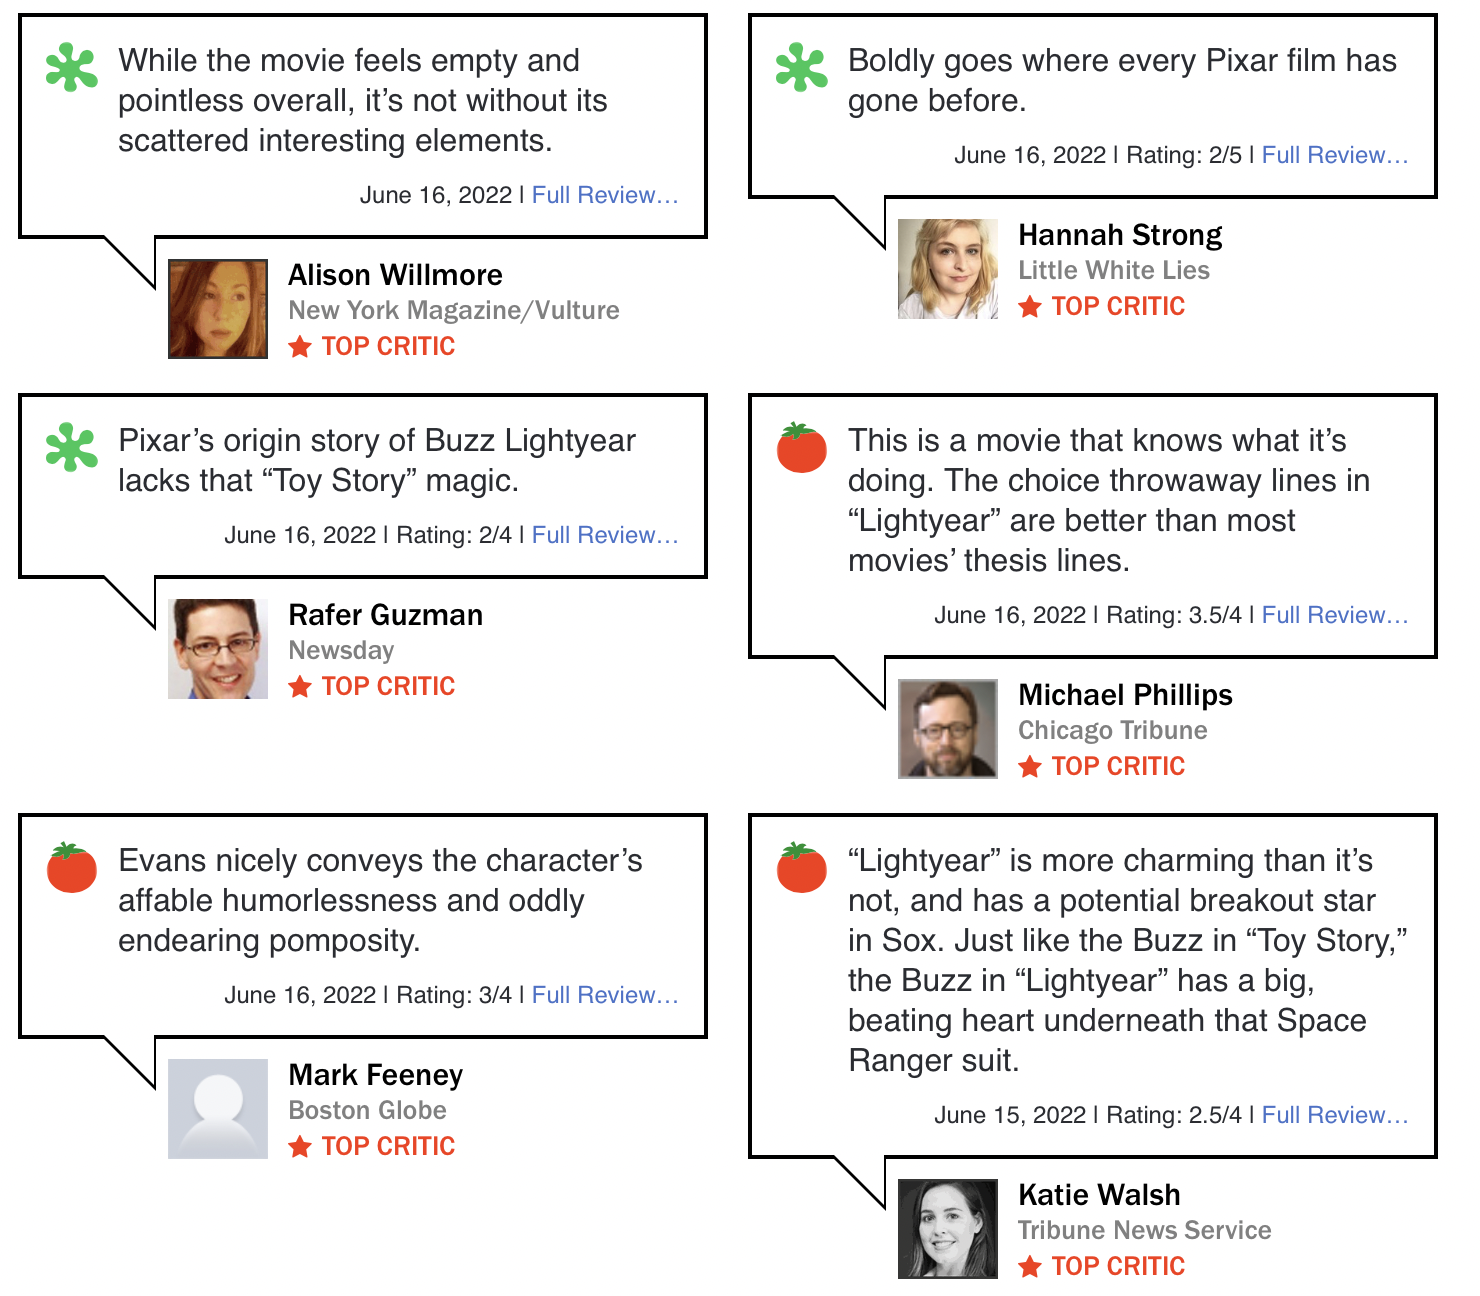
\includegraphics[scale=0.25]{img/rotten-tomatoes-comments.png}
    \caption{ Interfaz de comentarios de Rotten Tomatoes }\label{fig:rotten_tomatoes}
\end{figure}

\subsection{Letterboxd}

Por su parte, \href{https://letterboxd.com}{Letterboxd} sí que se siente más como una red social centrada en las
reseñas. Dándoles más importancia en el feed principal de la aplicación, en el que aparecen tanto las reseñas populares
entre demás usuarios y las de los usuarios que tú sigues. También permite comentar las reseñas de los demás usuarios.
Además, ofrece información sobre las distintas películas de la base de datos. De esta forma, Letterboxd se ofrece como
una solución mucho más acertada a los problemas planteados en este proyecto.\\
\begin{figure}[H]
    \centering	
    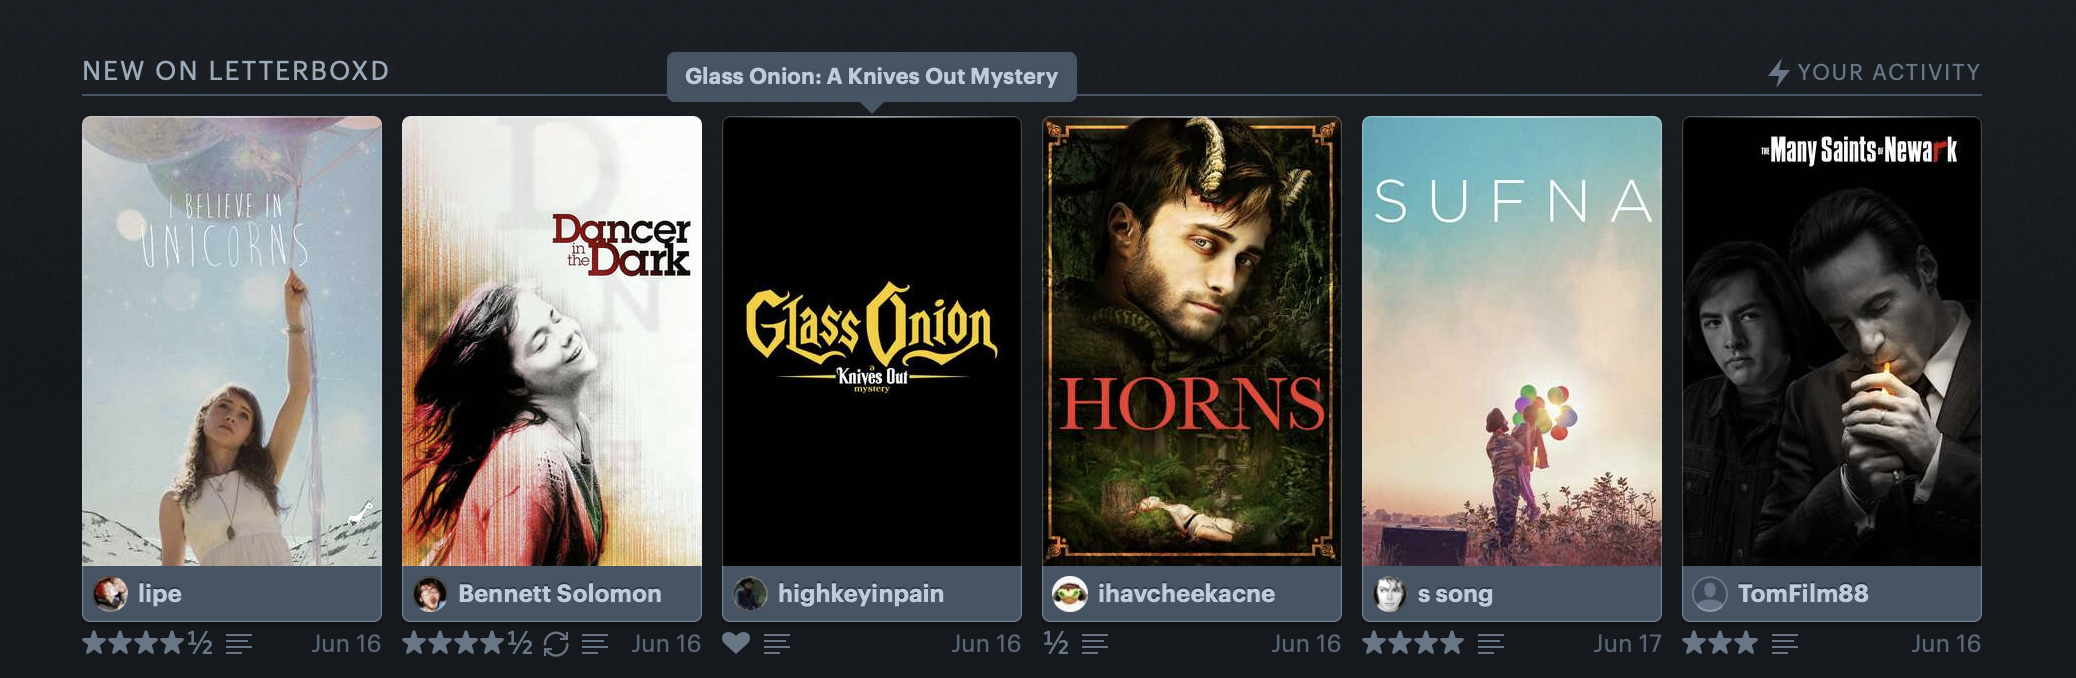
\includegraphics[scale=0.4]{img/letterboxd-feed.png}
    \caption{ Feed de la aplicación Letterboxd }\label{fig:letterboxd}
\end{figure}

Entonces, ¿por qué realizar una nueva aplicación? Los dos inconvenientes de Letterboxd son su interfaz algo desfasada
y que solo permite realizar reseñas de películas, por lo que nuestros usuarios \textit{seriéfilos} son dejados de lado
en esta aplicación.\\

\section{Mi propuesta ante el estado del arte}

Tras analizar las soluciones existentes y contrastarlas con los \hyperref[sec:objetivo]{objetivos} y requisitos de los
\hyperref[chap:personas]{usuarios} del proyecto, he obtenido una serie de conocimientos que me permitirán desarrollar
una solución que no cometa los mismos fallos que el resto. \\

Para cerrar el capítulo, expondré brevemente los puntos por los que ha de guiarse la solución. 
\begin{itemize}
    \item Feed de la aplicación centrado en las reseñas, mostrando las reseñas de usuarios populares y de los usuarios
    que sigues.
    \item Permitir comentar sobre las reseñas de otros usuarios, dando mayor sensación de red social.
    \item Cobertura tanto a películas como a series.
    \item Interfaz moderna, agradable a la vista y user-friendly.
\end{itemize}